
\chapter{部署文档}

\section{项目背景}

\subsection{市场需求分析}
随着互联网技术的飞速发展和人们生活节奏的加快,外卖订餐服务已成为现代都市生活中不可或缺的一部分。越来越多的人选择通过手机应用程序或网站来订购美食,享受便捷的送餐服务。据统计,近年来外卖市场呈现出快速增长的趋势,市场规模不断扩大,用户数量持续攀升。因此,开发一款高质量的在线订餐平台具有巨大的市场需求和发展潜力。

\subsection{用户痛点分析}
尽管市场上已经存在多家知名的外卖平台,但在实际使用过程中,用户仍然面临诸多不便:
\subsubsection{选择困难}
面对众多的餐厅选项,用户往往难以快速做出决策。
\subsubsection{配送延迟}
高峰时段订单量大,导致配送时间延长,影响用餐体验。
\subsubsection{食品安全}
部分小餐馆卫生条件差,食品质量难以保证。
\subsubsection{个性化推荐不足}
现有的推荐算法不够精准,无法满足用户的个性化需求。

\subsection{商家需求分析}
对于餐饮商家而言,加入一个高效的外卖平台同样具有重要意义:
\subsubsection{拓宽销售渠道}
通过线上平台吸引更多的顾客,提高销售额。
\subsubsection{降低运营成本}
减少线下宣传费用,利用平台流量优势增加曝光度。
\subsubsection{提升服务质量}
借助平台提供的数据分析工具,优化菜品结构和服务流程。

\subsection{项目目标}
基于以上分析,“饿了吧”项目旨在打造一个高效、便捷且安全的在线订餐平台,具体目标包括:
\subsubsection{丰富菜品选择}
整合周边优质餐厅资源,提供多样化的菜品供用户选择。
\subsubsection{优化配送流程}
引入先进的物流管理系统,缩短配送时间,提升用户体验。
\subsubsection{保障食品安全}
严格筛选合作商家,确保所有上线餐厅均符合卫生标准。
\subsubsection{智能推荐系统}
利用大数据分析技术,根据用户喜好和历史订单记录进行个性化推荐。

通过实现这些目标,“饿了吧”项目将为用户提供更加优质的订餐体验,同时也为商家带来更多的商业机会,实现双赢的局面。


\section{系统需求}



\section{项目部署的系统需求}

\subsection{前端系统需求}
\subsubsection{操作系统}
- 支持主流的操作系统,包括 Windows、macOS 和 Linux。

\subsubsection{浏览器兼容性}
- 支持最新版本的 Chrome、Firefox、Safari 和 Edge 浏览器。

\subsubsection{移动设备}
- 支持 iOS 和 Android 操作系统的移动设备。

\subsection{后端系统需求}
\subsubsection{服务器配置}
- CPU:至少 2 核心

- 内存:至少 2 GB

- 硬盘:至少 5 GB 可用空间

\subsubsection{数据库}
- MySQL 5.7 或更高版本

\subsubsection{中间件}
- Nginx 作为反向代理服务器

- Redis 用于缓存和会话管理

- RabbitMQ 用于消息队列

\subsubsection{其他依赖}
- Java 8 或更高版本

- Spring Boot

- Maven

\subsection{网络需求}

\subsubsection{IP 地址}
- 具备公网 IP 地址,以便外部访问。

\subsection{安全性需求}
\subsubsection{数据加密}
- 使用 HTTPS 协议,确保数据传输的安全性。

\subsection{运维需求}

\subsubsection{持续集成/持续部署 (CI/CD)}
- 使用 宝塔面板 实现构建、测试和部署流程。

\subsubsection{日志管理}
- 收集和分析系统日志,快速定位问题。


\section{配置说明}

\subsection{数据库配置}

\subsubsection{数据库类型}
- MySQL

\subsubsection{数据库连接信息}
- 主机:http://140.143.151.181/

- 端口:3306

- 数据库名称:elm

- 用户名:admin

- 密码:123456


\subsubsection{数据库表结构}

\begin{figure}[H]
  \centering
  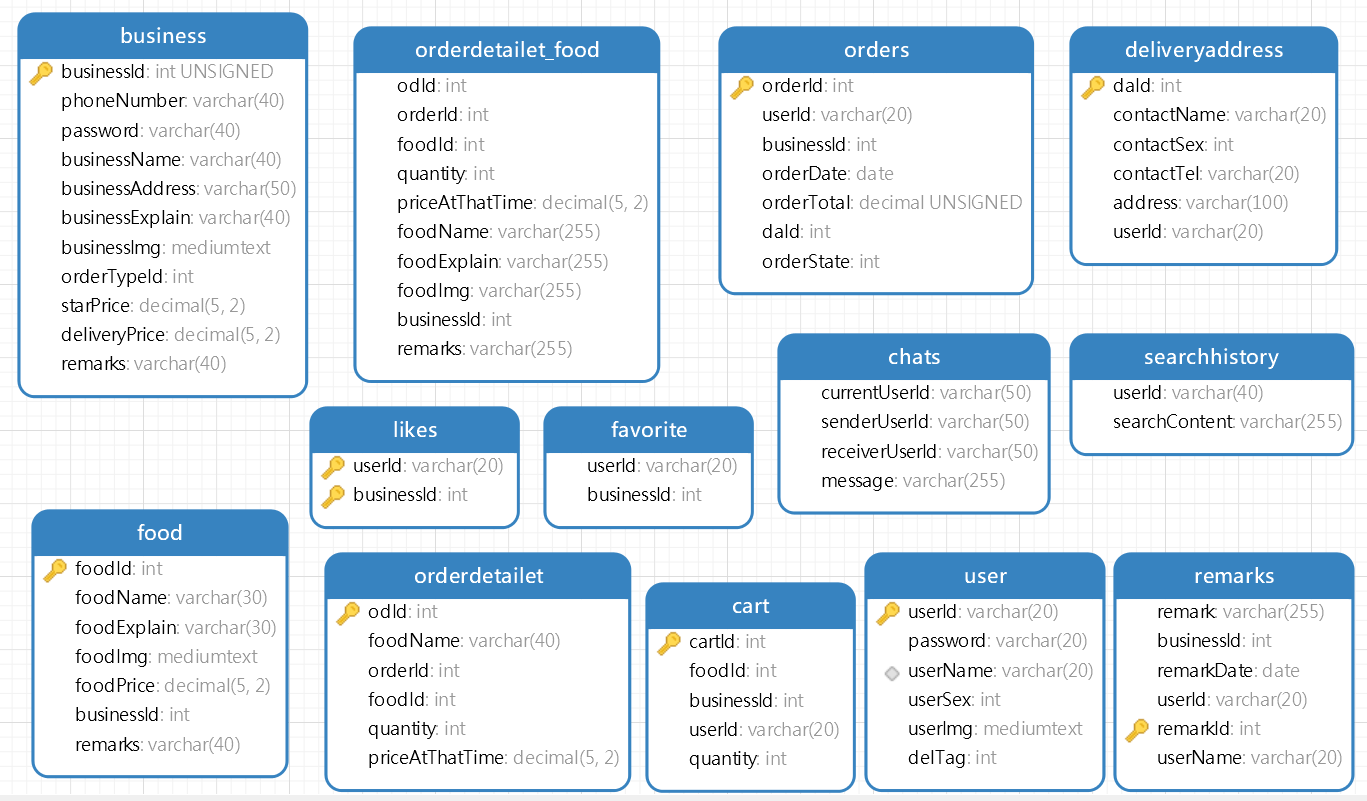
\includegraphics[width=1\textwidth]{Picture20}
  \caption{数据库表结构}\label{fig:xml}
  \vspace{\baselineskip}
\end{figure}



\section{部署的步骤和流程}

\subsection{服务器配置}
\begin{enumerate}
  \item 安装 Ubuntu 20.04 LTS 服务器。
  \item 安装 Nginx 和 MySQL。
  \item 安装 Java 和 Spring Boot。
  \item 安装 Redis 和 RabbitMQ。
\end{enumerate}
\subsection{前端部署}
\begin{enumerate}
  \item 将前端代码部署到服务器上。
  \item 配置 Nginx,将前端请求重定向到服务器。
\end{enumerate}
\subsection{后端部署}
\begin{enumerate}
  \item 将后端代码部署到服务器上。
  \item 配置 Nginx,将后端请求重定向到服务器。
\end{enumerate}
\subsection{数据库部署}
\begin{enumerate}
  \item 将数据库部署到服务器上。
\end{enumerate}
\subsection{其他配置}
\begin{enumerate}
  \item 安装宝塔面板,方便操作
  \item 配置 Nginx,将前端和后端请求重定向到服务器。
  \item 配置日志管理,快速定位问题。
\end{enumerate}